\begin{frame}{Finite State Entropy}
  \begin{itemize}
    \item \textbf{Limita Huffman}: Alocă un număr întreg de biți per simbol. Pentru
      simboluri dominante ($P > 0.5$), acest fapt introduce redundanță față de entropia sursei.

    \item \textbf{Mecanismul FSE (ANS)}: Absoarbe probabilitățile într-un automat finit determinist,
      permițând reprezentarea simbolurilor folosind o \textbf{medie fracționară de biți}.
  \end{itemize}

  \vspace{0.2cm}
  \textbf{Cum se realizează compresia?} Intervalul finit al stărilor $[0, 2^{k}- 1]$ este partiționat
  proporțional cu probabilitatea fiecărui simbol. Simbolurile frecvente primesc o plajă
  mai mare de stări, necesitând \textbf{mai puțini biți} extrași din flux pentru
  renormalizare.

  \vspace{0.4cm}
  \begin{center}
    \resizebox{0.85\linewidth}{!}{%
    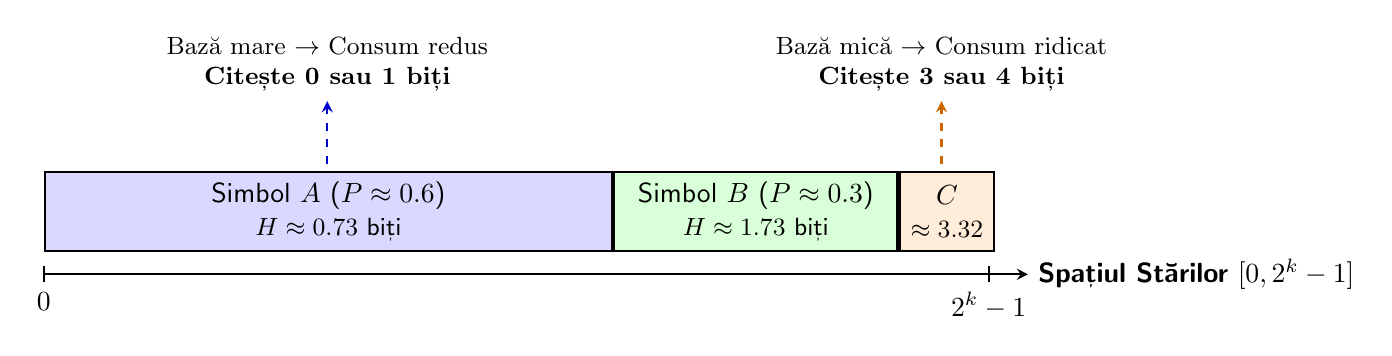
\begin{tikzpicture}[
      font=\sffamily,
      thick,
      bar/.style={draw=black, minimum height=1.0cm, align=center}, % redus de la 1.5cm
      freq/.style={fill=blue!15},
      mid/.style={fill=green!15},
      rare/.style={fill=orange!15}
    ]
      % The main state space bar
      % Total width = 12cm for visual scale
      % A: prob 0.6 (7.2cm), B: prob 0.3 (3.6cm), C: prob 0.1 (1.2cm)
      \node[bar, freq, minimum width=7.2cm, anchor=west]
        (A)
        at
        (0,0)
        {Simbol $A$ ($P \approx 0.6$) \\ \small $H \approx 0.73$ biți};

      \node[bar, mid, minimum width=3.6cm, anchor=west]
        (B)
        at
        (A.east)
        {Simbol $B$ ($P \approx 0.3$) \\ \small $H \approx 1.73$ biți};

      \node[bar, rare, minimum width=1.2cm, anchor=west]
        (C)
        at
        (B.east)
        {$C$ \\ \small $\approx 3.32$};

      % Axis below (mutat mai aproape de blocuri: -0.8 în loc de -1.2)
      \draw[->, >=stealth, thick]
        (0, -0.8) -- (12.5, -0.8)
        node[right] {\textbf{Spațiul Stărilor} $[0, 2^{k}-1]$};
      \draw[thick] (0, -0.7) -- (0, -0.9) node[below] {$0$};
      \draw[thick] (12, -0.7) -- (12, -0.9) node[below] {$2^{k}-1$};

      % Annotation arrows showing bitstream consumption (scurtate)
      \draw[->, >=stealth, blue!80!black, dashed, thick]
        (3.6, 0.6) -- (3.6, 1.4)
        node[above, text=black, align=center, font=\small]
          {Bază mare $\to$ Consum redus \\ \textbf{Citește 0 sau 1 biți}};

      \draw[->, >=stealth, orange!80!black, dashed, thick]
        (11.4, 0.6) -- (11.4, 1.4)
        node[above, text=black, align=center, font=\small]
          {Bază mică $\to$ Consum ridicat \\ \textbf{Citește 3 sau 4 biți}};
    \end{tikzpicture}%
    }
  \end{center}
\end{frame}